\documentclass[dvipsnames,tikz]{standalone}
\usepackage{amsmath}
\usepackage{arevmath}
\usepackage{xcolor}
\usepackage{tikz}
\usetikzlibrary{calc}
\usetikzlibrary{decorations.pathreplacing,calligraphy,3d}

\tikzset{main/.style={draw=black, circle, color=black}}


\begin{document}
	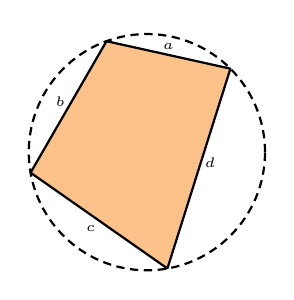
\begin{tikzpicture}[scale=0.75, main, line join=bevel]
		\fill[BurntOrange, semitransparent] (45:2) -- (110:2) -- (190:2) -- (280:2) -- cycle;
		\draw[thick, densely dashed] (0,0) circle (2cm);
		\draw[thick, main] (45:2) -- (110:2) -- (190:2) -- (280:2) -- cycle;
		\draw[font=\tiny, main] (45:2) to node [midway, yshift=3pt] {$a$} (110:2);
		\draw[font=\tiny, main] (110:2) to node [midway, xshift=-3pt, yshift=2pt] {$b$} (190:2);
		\draw[font=\tiny, main] (190:2) to node [midway, xshift=-3pt, yshift=-3pt] {$c$} (280:2);
		\draw[font=\tiny, main] (280:2) to node [midway, xshift=4pt, yshift=2pt] {$d$} (45:2);
	\end{tikzpicture}
\end{document}